\documentclass{article}
\usepackage{graphicx}
\usepackage[utf8]{inputenc}
\usepackage[spanish]{babel}
\begin{document}

\begin{figure}
    \centering
    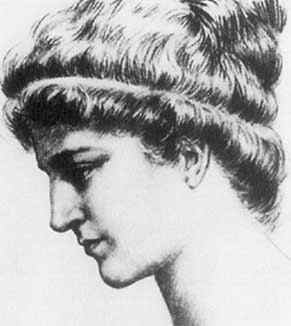
\includegraphics[width=.6\textwidth]{Hypatia.jpeg}
    
    \label{fig:my_label}
\end{figure}

{\centering \textbf {Hipatia de Alejandría}\par}

\vspace{20mm}

 Fue una Matemática, filósofa y maestra neoplatónica griega, natural de Egipto, que destacó en los campos de las matemáticas y la astronomía, miembro y cabeza de la Escuela neoplatónica de Alejandría a comienzos del siglo v. Seguidora de Plotino, cultivó los estudios lógicos y las ciencias exactas, llevando una vida ascética. Fue la primera mujer en hacer una contribución sustancial al desarrollo de las matemáticas.
\vspace{5mm}

No hay evidencia de que Hypatia haya realizado una investigación matemática original. Sin embargo, ella ayudó a su padre Theon de Alejandría al escribir su comentario de once partes sobre \emph{Ptolomeo Almagesto} También se cree que ella también ayudó a su padre a producir una nueva versión de \emph{Elementos de Euclides} que se ha convertido en la base de todas las ediciones posteriores de Euclides.
\vspace{5mm}

Ninguna de sus obras se ha conservado, pero se conocen gracias a sus discípulos, como Sinesio de Cirene o Hesiquio de Alejandría, el Hebreo.


\end{document}